
\begin{figure}[H]
\centering
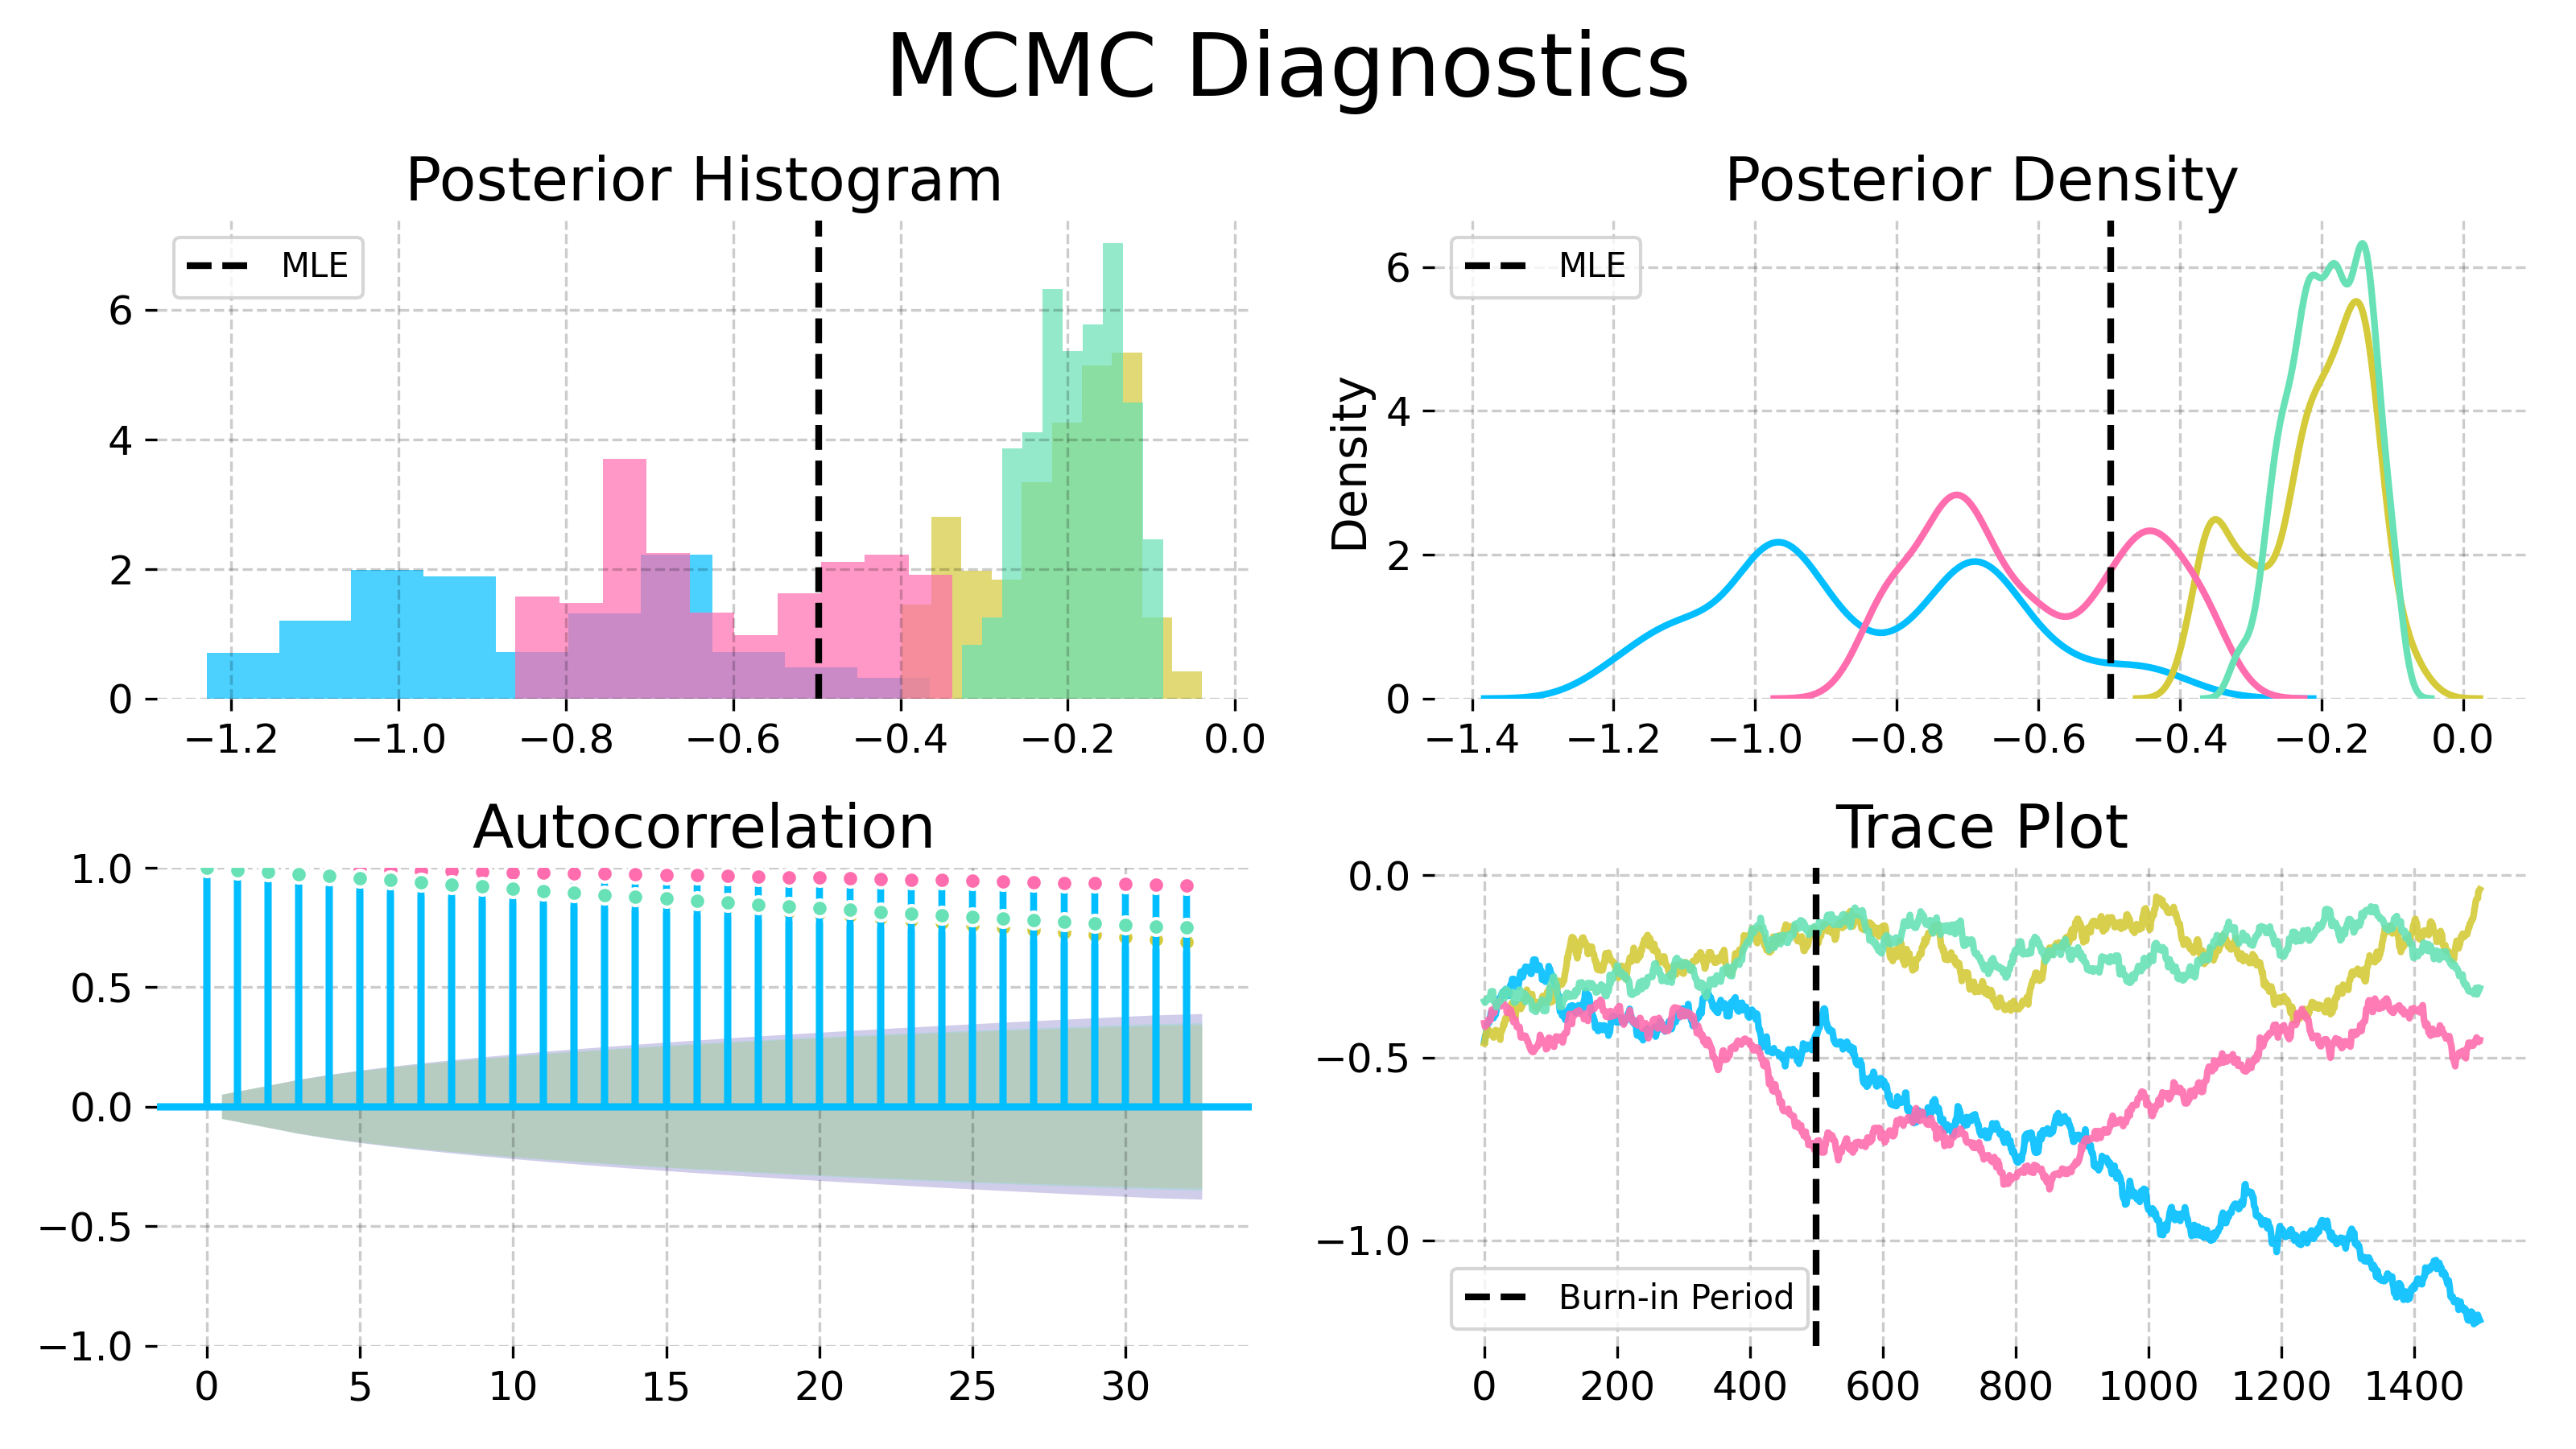
\includegraphics[width=\textwidth/\real{1.25}]{imgs/pmcmc/mh.png}
\caption{
  Convergence diagnostics for the Metropolis-Hastings variant particle MCMC with the random walk proposal and an informative empirical prior from IF2.
  Here, we display the results for the trend parameter in the Dhaka cholera model of \cite{king08}.
  The poor convergence shown here, using an MCMC algorithm that does not have access to derivatives, contrasts with Fig.~\ref{fig:nuts-eb} in the main text.
}
    \label{fig:mh}
\end{figure}
\FloatBarrier

%\newpage

\begin{figure}[H]
    \centering
    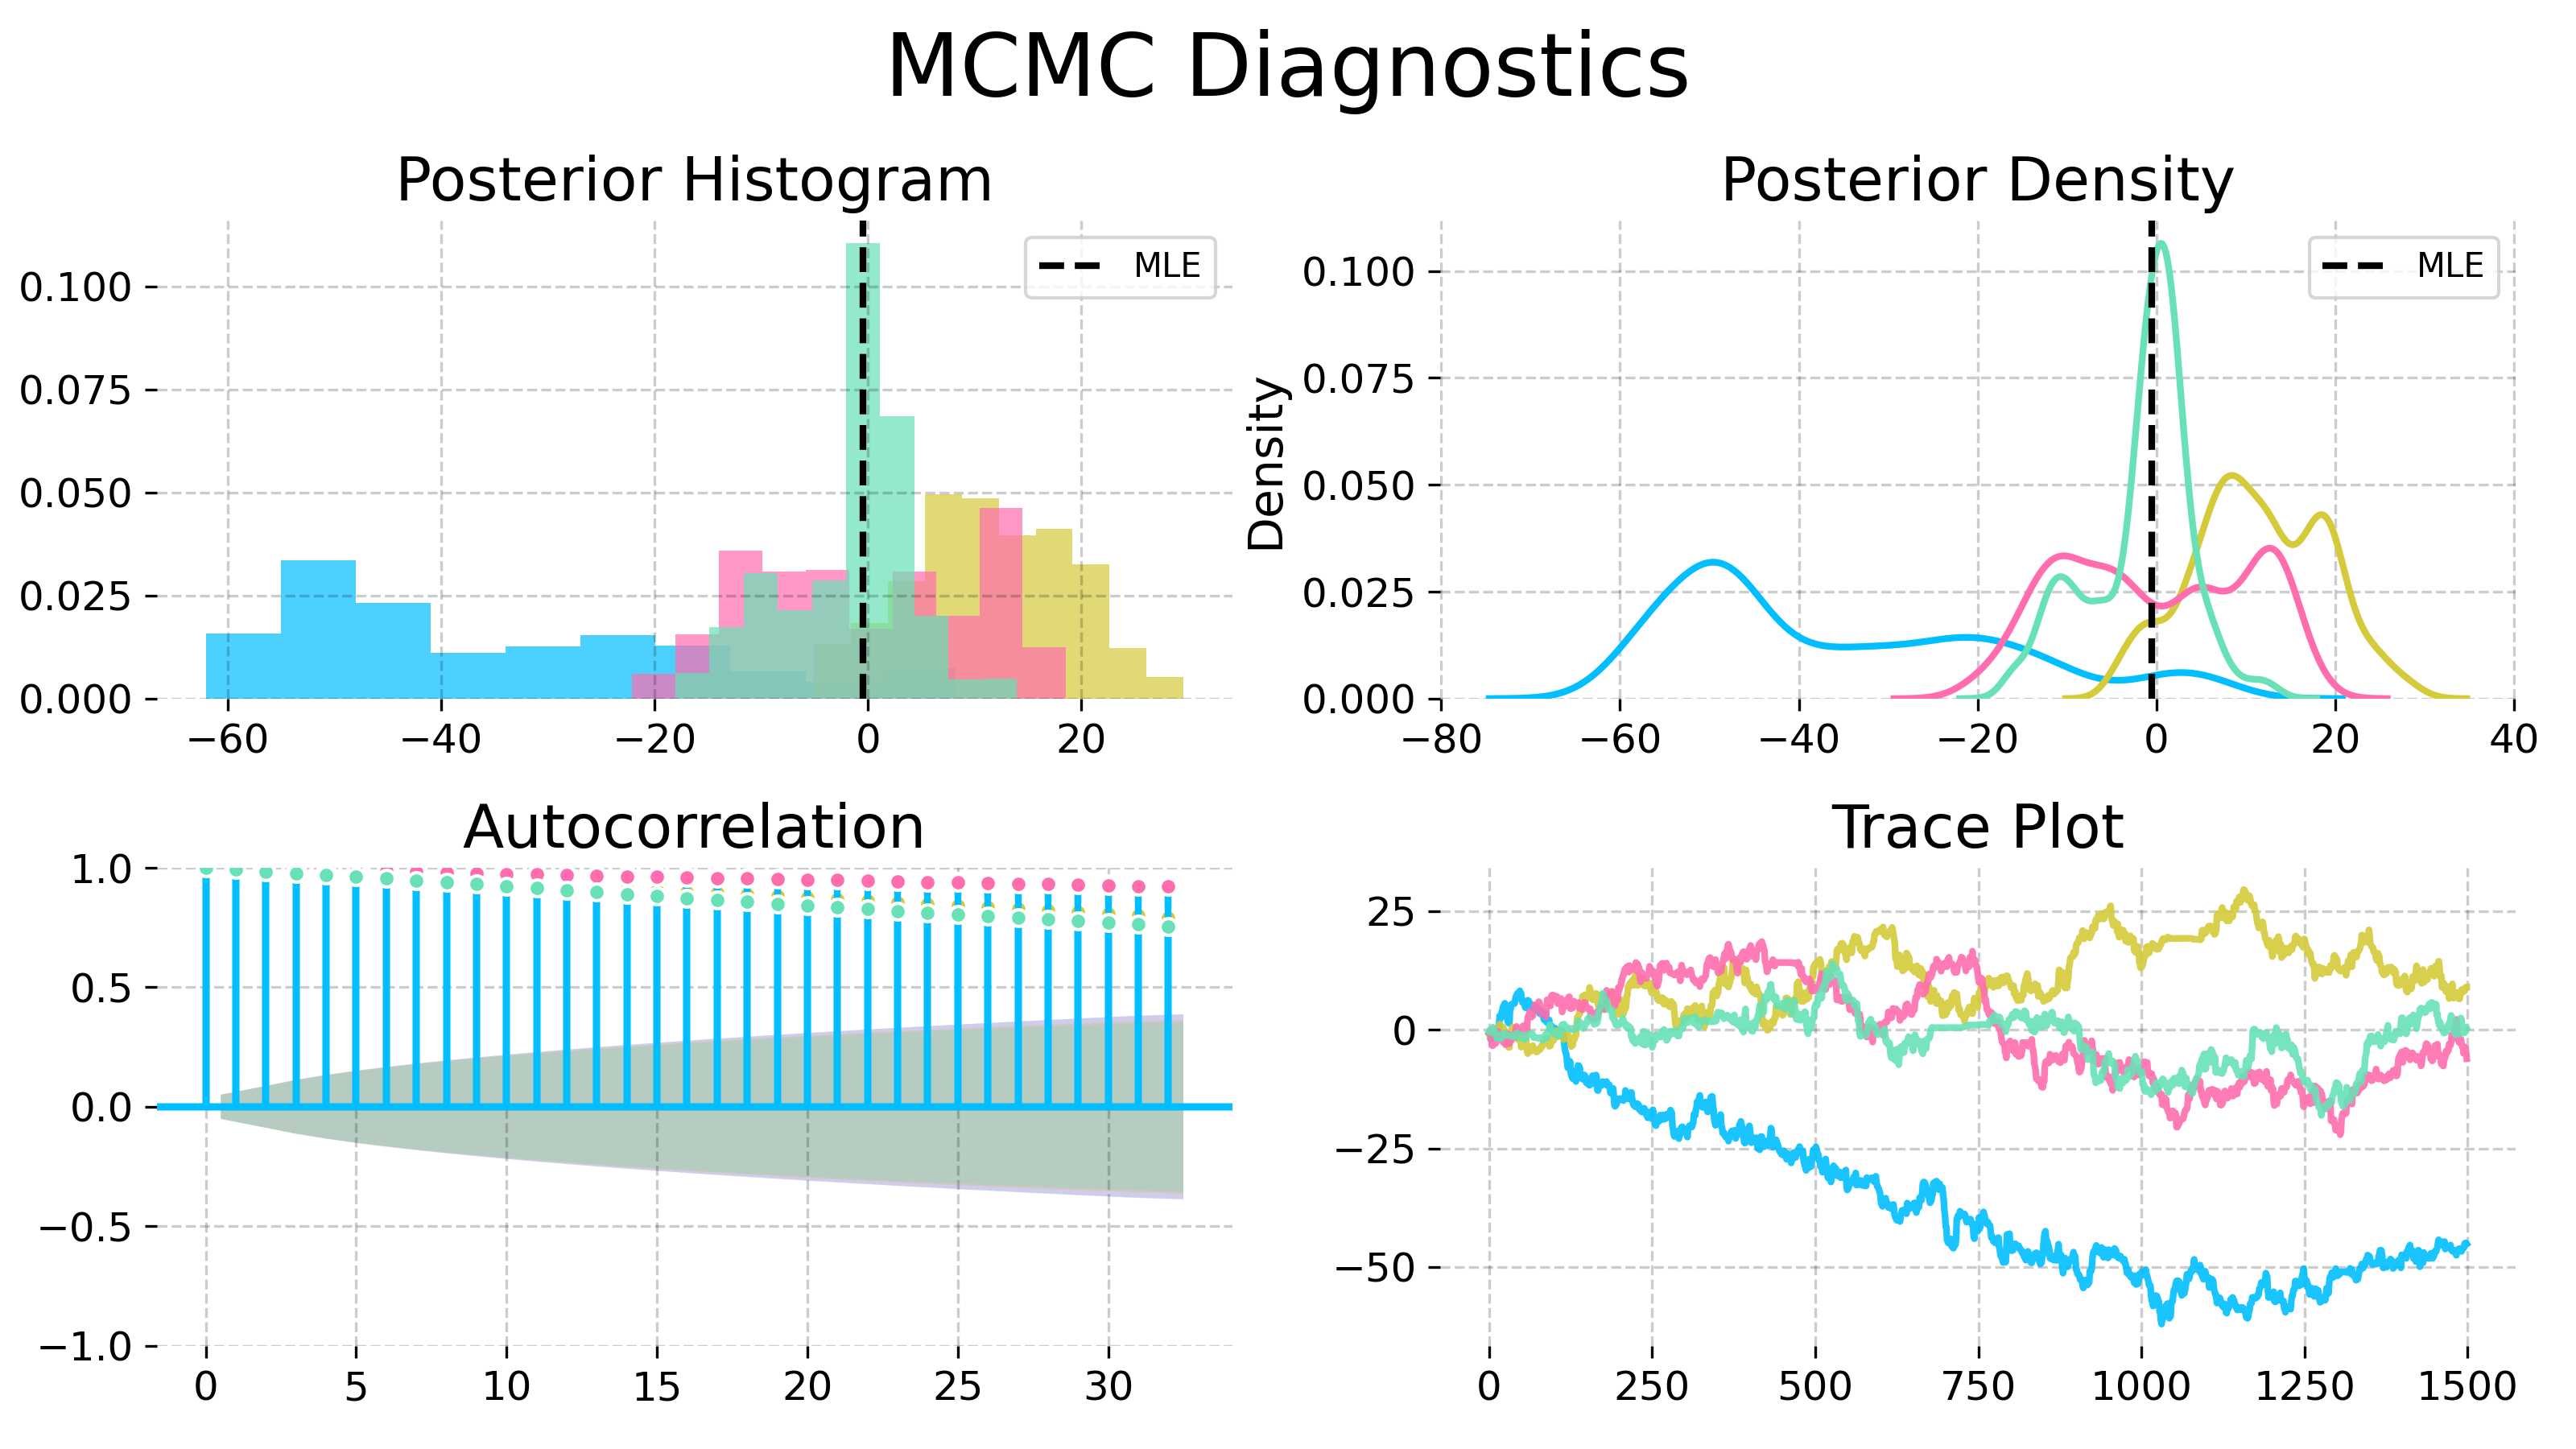
\includegraphics[width=\textwidth/\real{1.25}]{imgs/pmcmc/nuts.png}
    \caption{Convergence diagnostics for a No-U-Turn Sampler (NUTS) with uniform priors on a compact set. Again, we display the results for the trend parameter in the Dhaka cholera model of \cite{king08}. The NUTS sampler explores more of the posterior than the Metropolis-Hastings sampler, but fails to converge quickly.
      This poor convergence, compared with Fig.~\ref{fig:nuts-eb} in the main text, demonstrates the value of the empirical prior for obtaining successful convergence.
}
    \label{fig:nuts}
\end{figure}
\FloatBarrier
\newpage

\begin{figure}[H]
    \centering\
    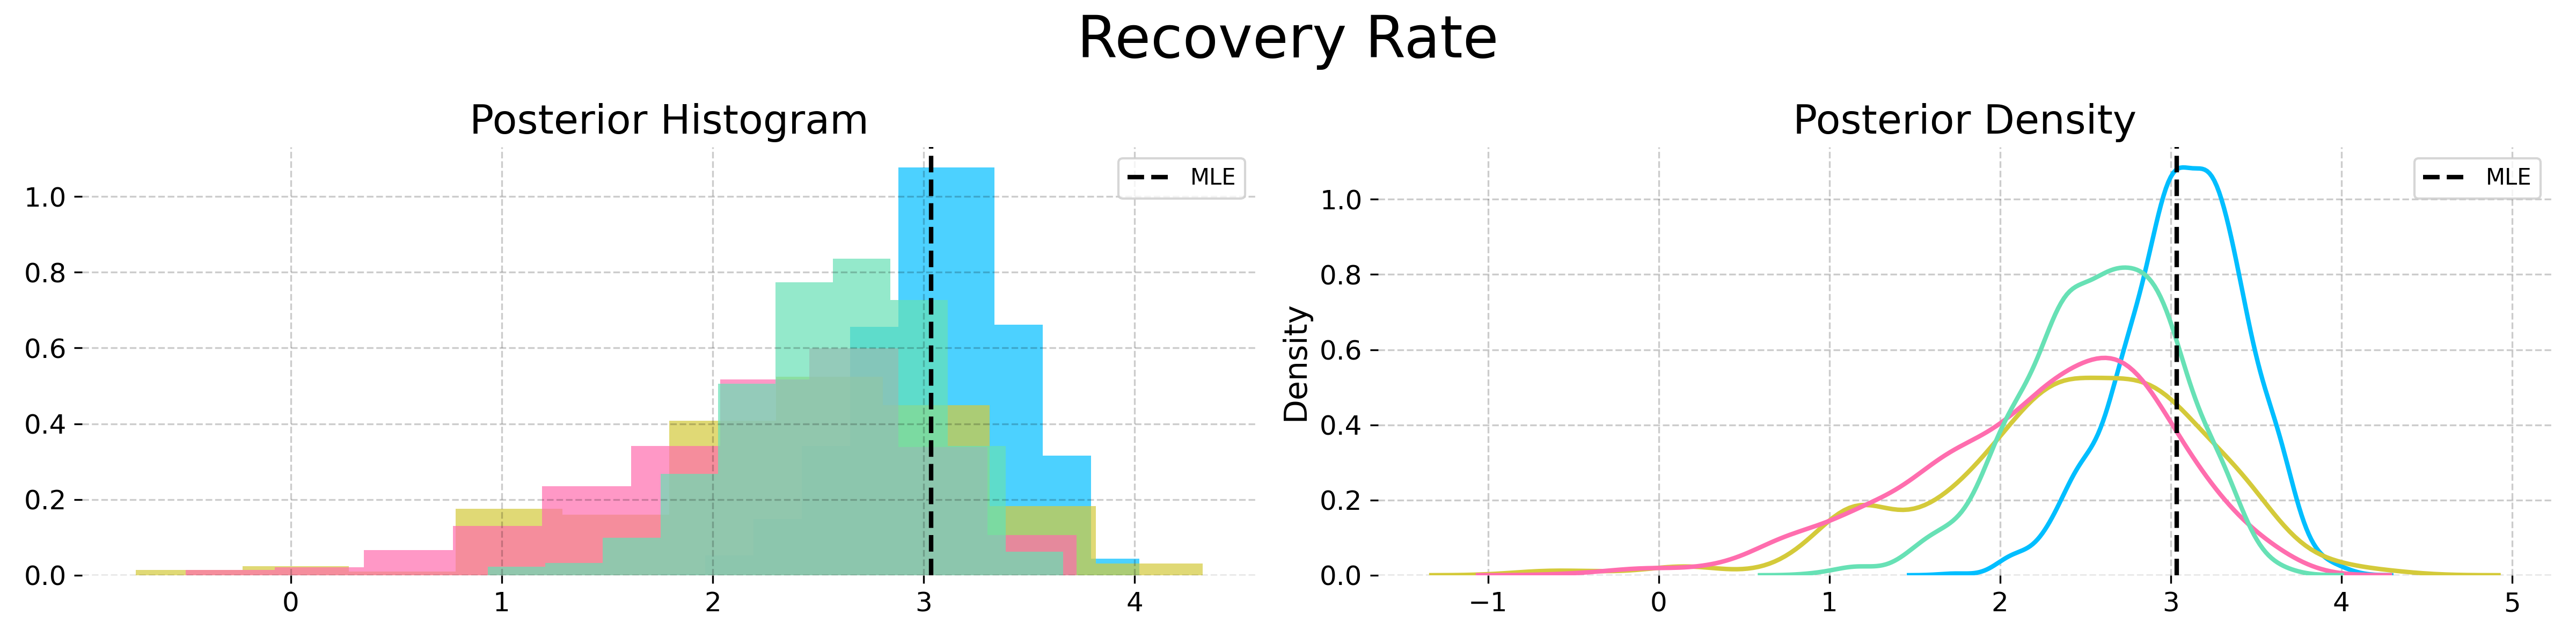
\includegraphics[scale=0.30]{imgs/pmcmc/nuts_eb/Recovery_Rate.png}
    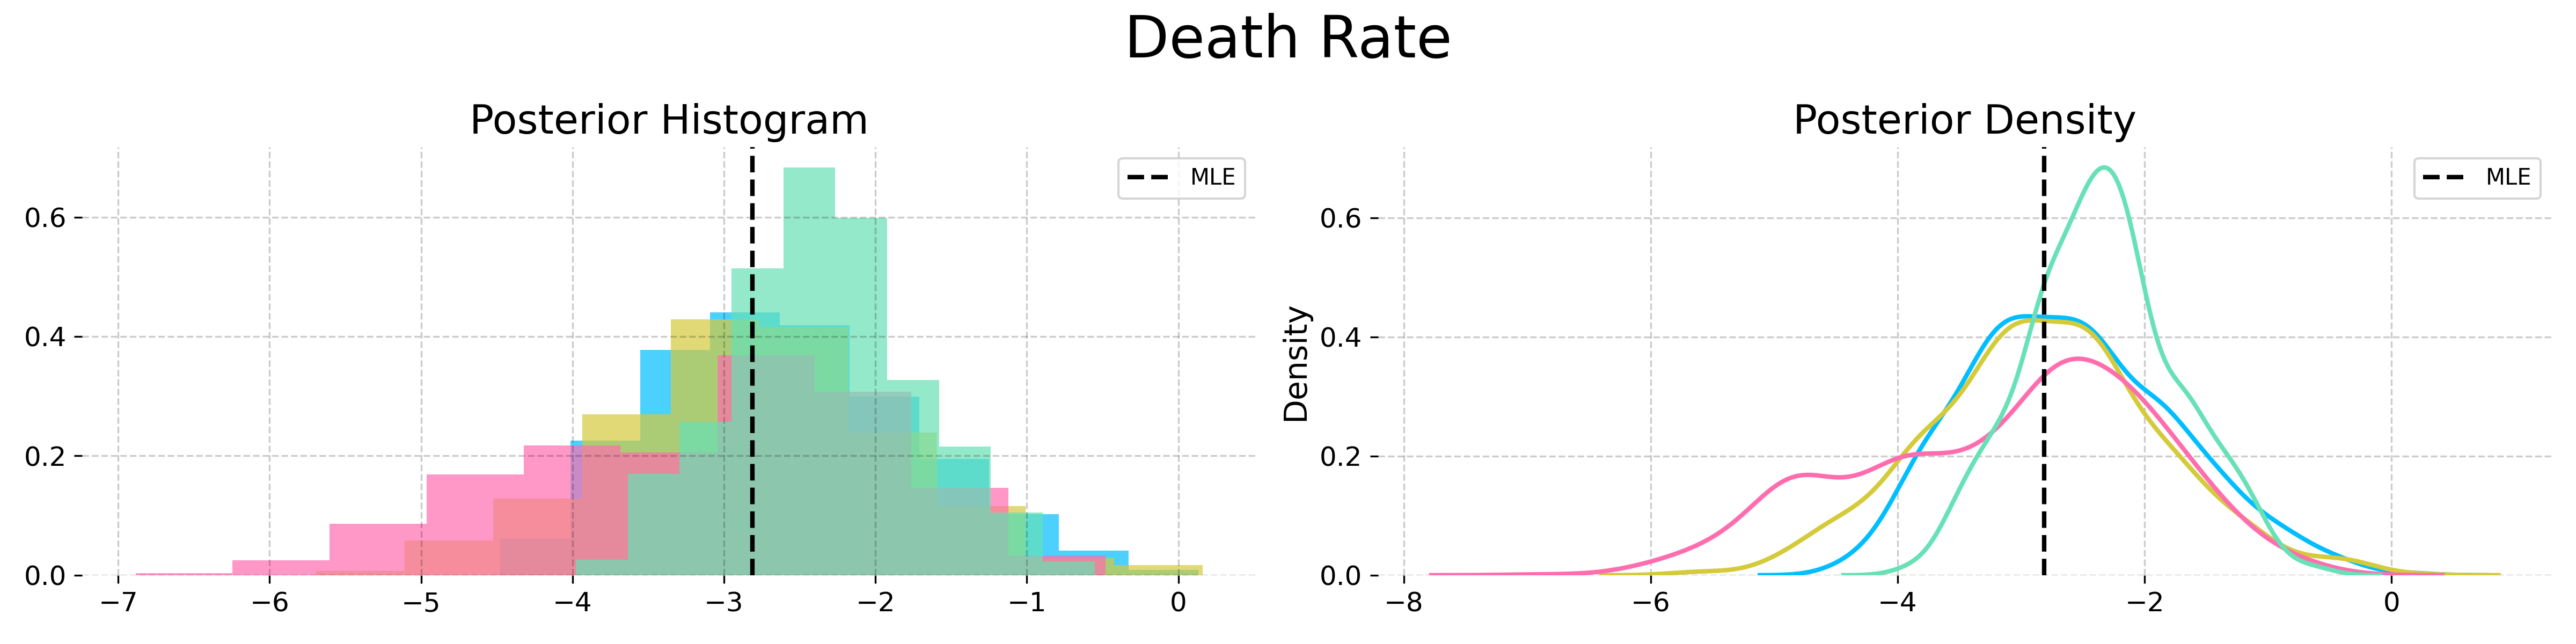
\includegraphics[scale=0.30]{imgs/pmcmc/nuts_eb/Death_Rate.png}
    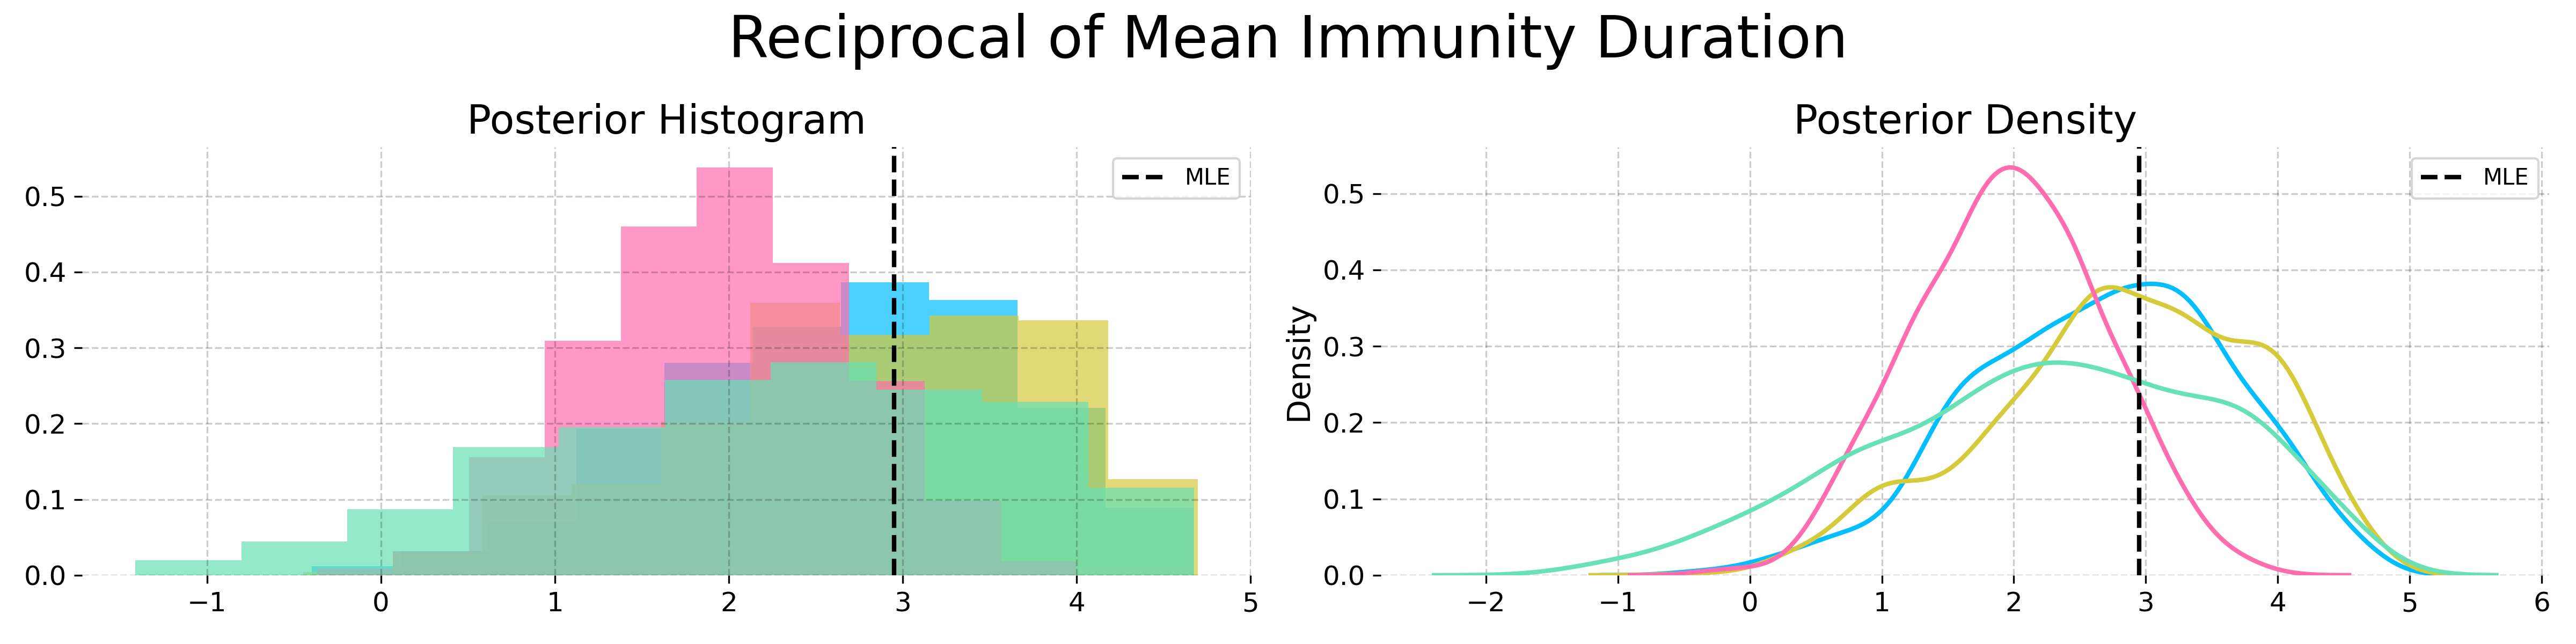
\includegraphics[scale=0.30]{imgs/pmcmc/nuts_eb/Reciprocal_of_Mean_Immunity_Duration.png}
    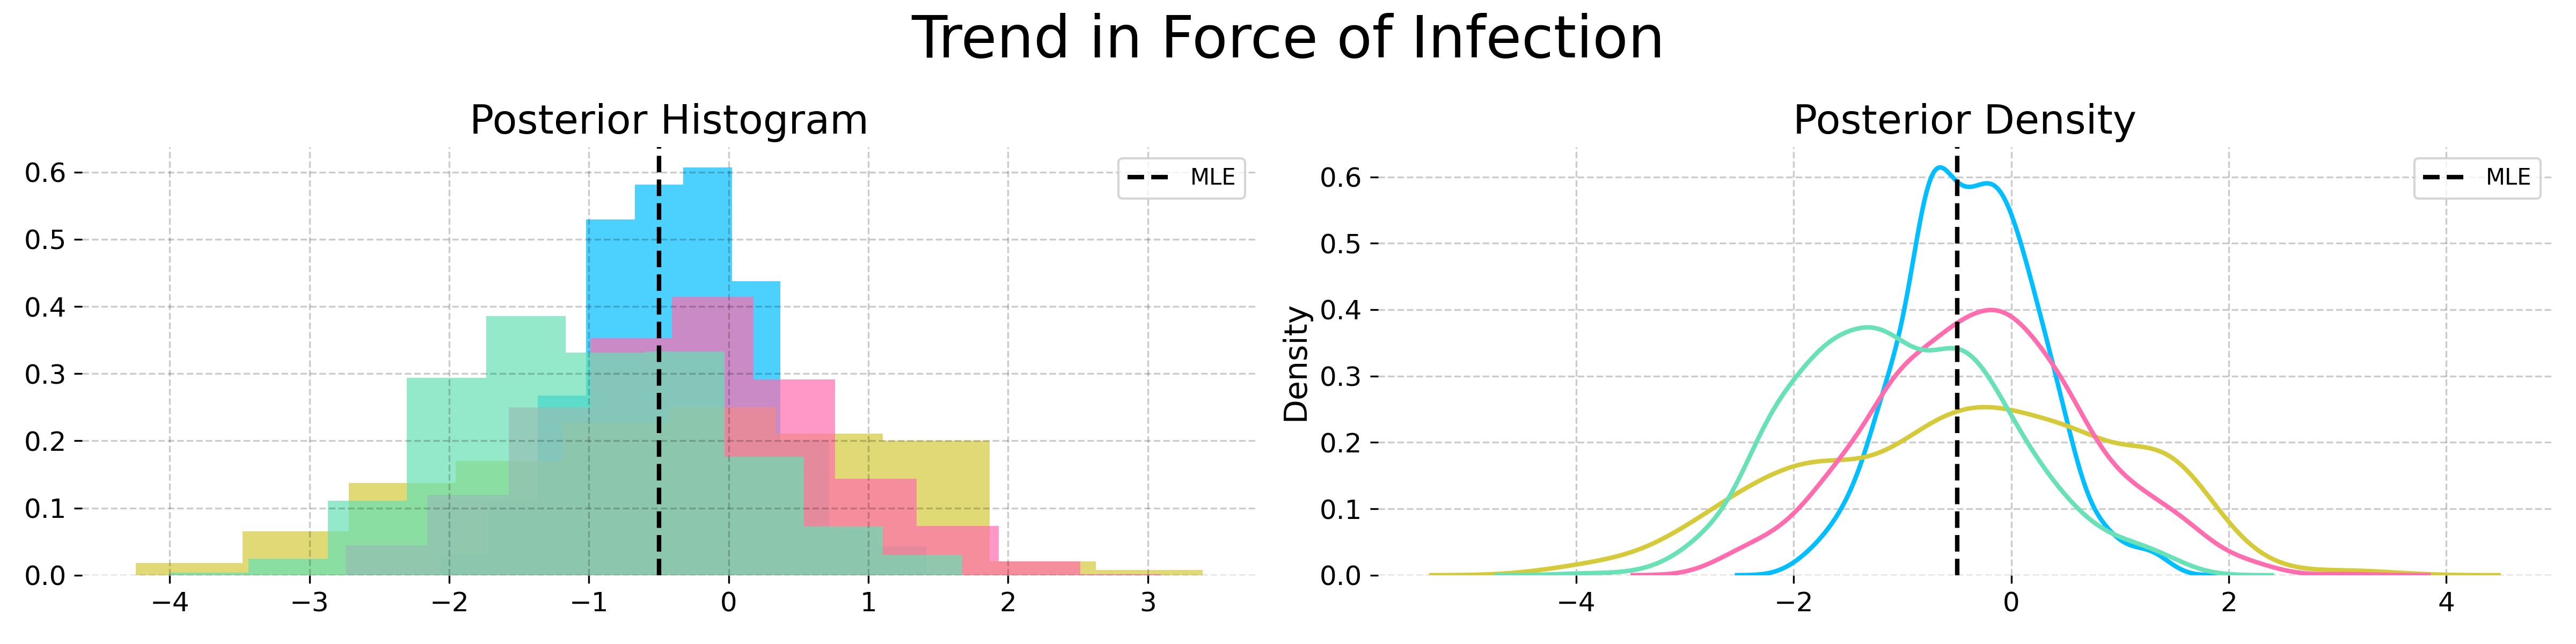
\includegraphics[scale=0.30]{imgs/pmcmc/nuts_eb/Trend_in_Force_of_Infection.png}
    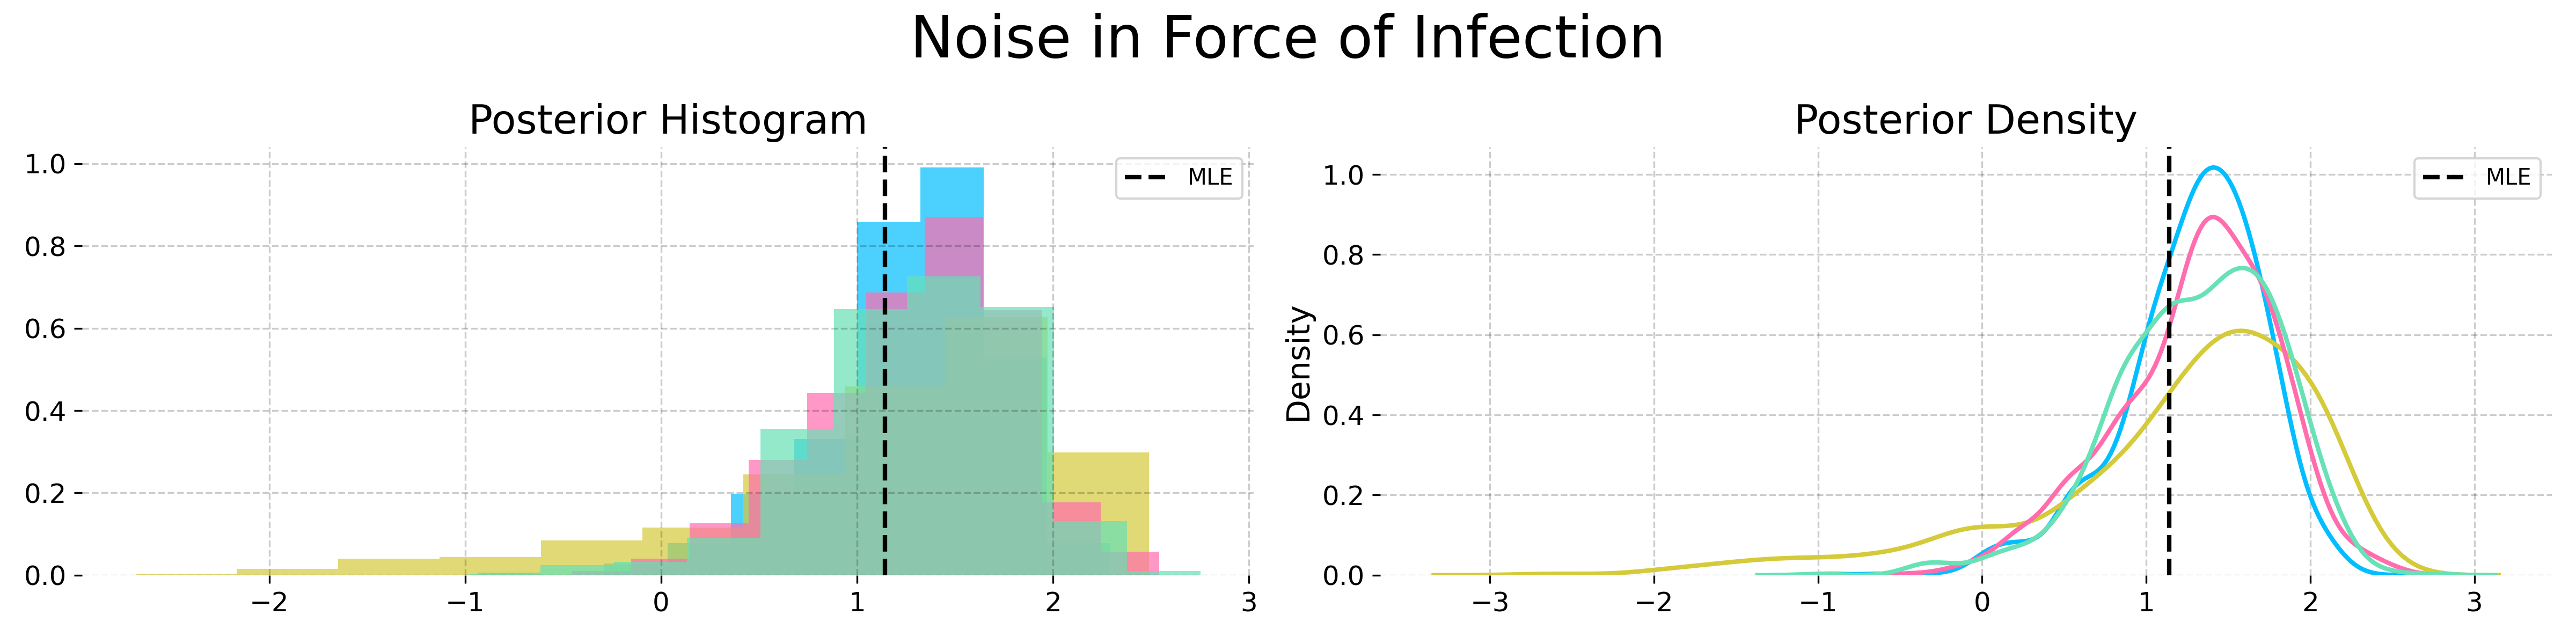
\includegraphics[scale=0.30]{imgs/pmcmc/nuts_eb/Noise_in_Force_of_Infection.png}
    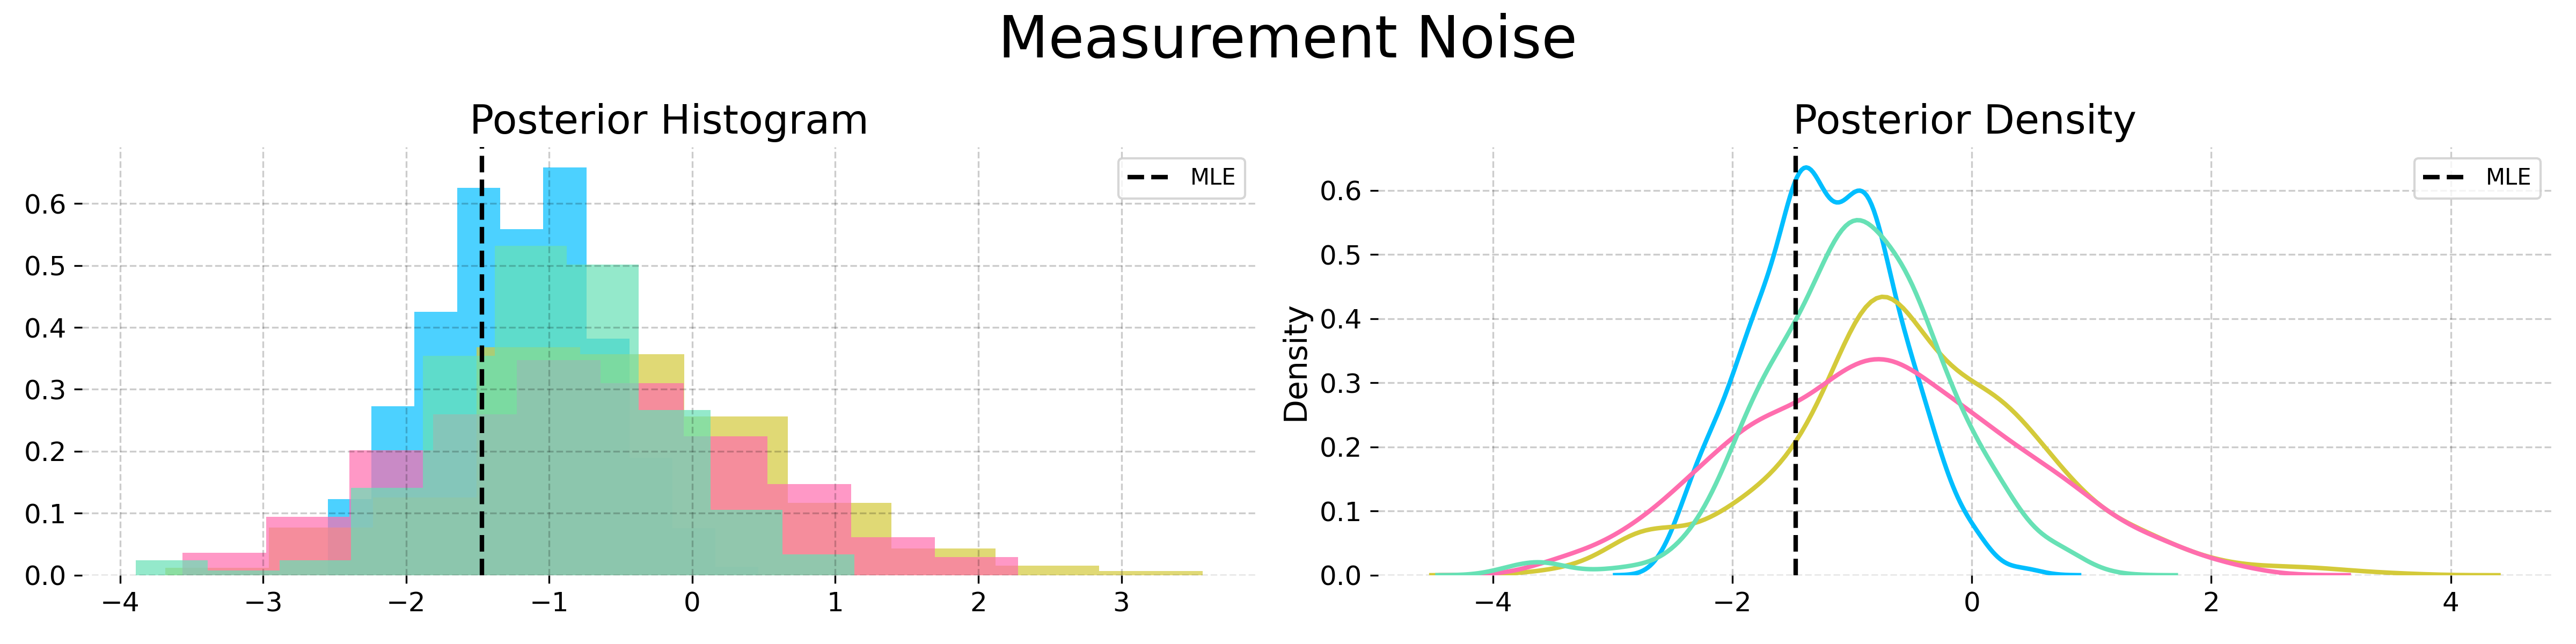
\includegraphics[scale=0.30]{imgs/pmcmc/nuts_eb/Measurement_Noise.png}
    \caption{Posterior estimates from NUTS powered by MOP-$\alpha$ with the informative nonparametric empirical prior obtained from a kernel density estimator on the IF2 parameter cloud. The posterior estimates from each chain are largely in agreement.}
    \label{fig:posteriors}
\end{figure}

\FloatBarrier
\newpage
